\chapter{Appendix \thechapter: Tables}\label{app:Tables}

\renewcommand\numberline[1]{\hbox to 56pt{Table #1:\hspace{1ex}}} % Add numbers and text to list of tables

\vspace*{-2.5cm}
\listofatables

\pagebreak

Testing the referencing command for this appendix... Reference Appendix \ref{app:Tables}.

\begin{atable}[htb]
    \caption{Table of Random Numbers}
    \label{tab:my_label4}
    \centering
    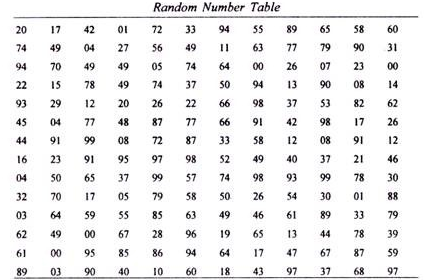
\includegraphics{tables/table.png}
\end{atable}

\newpage

\begin{atable}[htb]
    \caption{Table of Random Numbers}
    \label{tab:my_label5}    
    \centering
    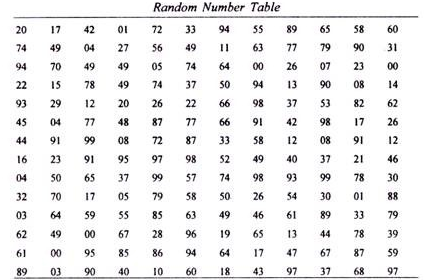
\includegraphics{tables/table.png}
\end{atable}


\pagebreak

%%%%%%%%%%%%%%%%%%%%%%%%%%%%%%%%%%%%%%%%%%%%%%%%%%%
%%%%%%%%%%%%%%%%%%%%%% NOTE %%%%%%%%%%%%%%%%%%%%%%%
%%%%%%%%%%%%%%%%%%%%%%%%%%%%%%%%%%%%%%%%%%%%%%%%%%%
% 
% Use \begin{atable} and \end{atable} for all tables that are included in the Tables Appendix section. This is to be able to generate a seperate list of tables.